\section{Auswertung}
\label{sec:Auswertung}
Allgemein lässt sich aus den Werten für die Anzahl $N$ der Impulse der Fehler
über
\begin{equation}
  \Delta N= \sqrt{N}
  \label{eqn:fehler}
\end{equation}
Bei der Nullmessung wird $N_u$=215 gemessen. Unter Berücksichtigung der Zeitspanne von
$\Delta t=900\;s$ und Gleichung \ref{eqn:fehler} ergibt sich als normierte Nullmessung:
\begin{equation}
  N_{un}=\SI{0,24(2)}.
\end{equation}

Die Ergebnisse der Messung Halbwertszeitmessung von Silber sind in Tabelle
\ref{tab:tab1} zu sehen. Diese werden zunächst in Abbildung \ref{fig:plot3}
halblogarithmisch gegen die Zeit $t$ aufgetragen.

\begin{table}[H]
  \centering
  \caption{Messwerte der Wärmepumpe}
  \label{tab:tabe1}
    \begin{tabular}{S S S S S S}
    \toprule
    $ t  \: / \si{\second} $ & $ p_a \: / \si{\bar} $ & $ p_b \: / \si{\bar} $ &
    $ T_1 \: / \si{\kelvin} $ & $ T_2 \: / \si{\kelvin} $ & $ P \: / \: \si{\watt} $\\
    \midrule
    0 & 5.0 & 5.0 & 293.65 & 293.65 & 0 \\
    60 & 4.7 & 6.0 & 294.15 & 293.55 & 115 \\
    120 & 4.4 & 6.4 & 295.15 & 293.15 & 118 \\
    180 & 4.5 & 6.9 & 296.35 & 291.95 & 122 \\
    240 & 4.6 & 7.0 & 297.55 & 290.95 & 125 \\
    300 & 4.6 & 7.0 & 298.85 & 289.95 & 125 \\
    360 & 4.5 & 7.2 & 300.05 & 289.15 & 123 \\
    420 & 4.4 & 7.4 & 301.15 & 288.45 & 123 \\
    480 & 4.3 & 7.8 & 302.35 & 287.65 & 122 \\
    540 & 4.2 & 8.0 & 303.55 & 286.95 & 122 \\
    600 & 4.2 & 8.1 & 304.65 & 286.25 & 121 \\
    660 & 4.1 & 8.3 & 305.75 & 285.55 & 121 \\
    720 & 4.0 & 8.5 & 306.75 & 284.95 & 121 \\
    780 & 4.0 & 8.8 & 307.75 & 284.35 & 121 \\
    840 & 3.9 & 9.0 & 308.75 & 283.75 & 121 \\
    900 & 3.8 & 9.1 & 309.65 & 283.15 & 121 \\
    960 & 3.8 & 9.2 & 310.55 & 282.55 & 122 \\
    1020 & 3.8 & 9.5 & 311.45 & 282.05 & 122 \\
    1080 & 3.7 & 9.8 & 312.25 & 281.55 & 122 \\
    1140 & 3.7 & 10.0 & 313.05 & 281.15 & 122 \\
    1200 & 3.7 & 10.0 & 313.9 & 280.65 & 122 \\
    1260 & 3.6 & 10.2 & 314.65 & 280.25 & 123 \\
    1320 & 3.6 & 10.3 & 315.35 & 279.85 & 123 \\
    1380 & 3.6 & 10.6 & 316.15 & 279.45 & 124 \\
    1440 & 3.6 & 10.8 & 316.85 & 279.15 & 124 \\
    1500 & 3.6 & 11.0 & 317.55 & 278.75 & 124 \\
    1560 & 3.6 & 11.1 & 318.25 & 278.55 & 124 \\
    1620 & 3.6 & 11.2 & 318.95 & 278.25 & 125 \\
    1680 & 3.5 & 11.4 & 319.55 & 277.95 & 125 \\
    1740 & 3.5 & 11.5 & 320.15 & 277.65 & 125 \\
    1800 & 3.5 & 11.7 & 320.75 & 277.45 & 125 \\
    1860 & 3.5 & 11.9 & 321.35 & 277.25 & 125 \\
    1920 & 3.5 & 12.0 & 321.95 & 277.05 & 125 \\
    1980 & 3.5 & 12.1 & 322.45 & 276.95 & 125 \\








      \bottomrule
    \end{tabular}
\end{table}


\begin{figure}[H]
  \centering
  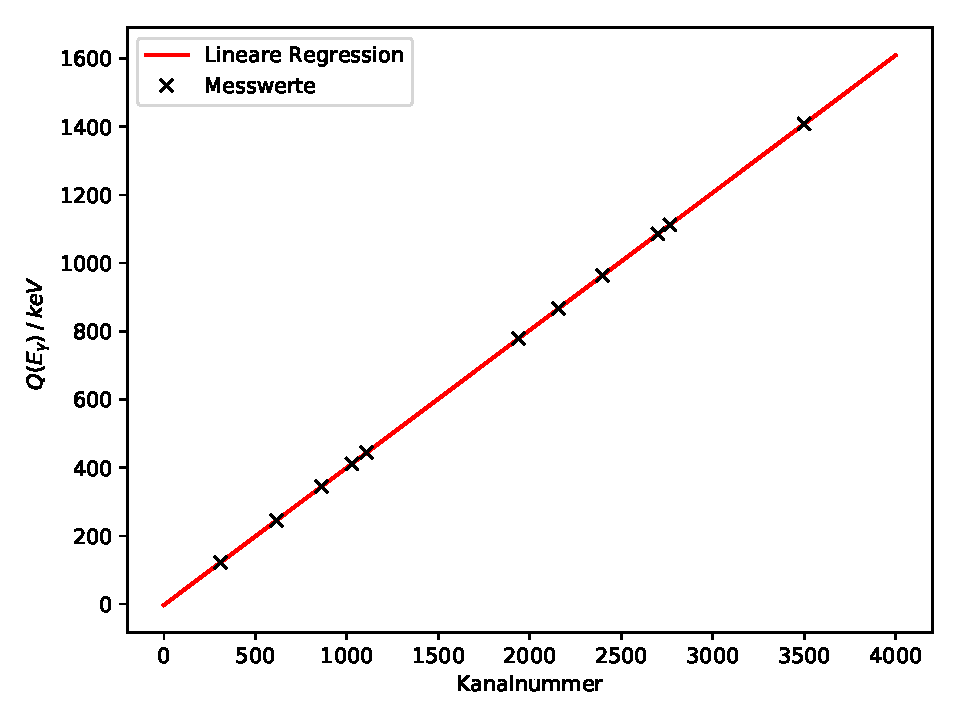
\includegraphics[height=7cm]{plot3.pdf}
  \caption{Halblogarithmisch aufgetragene Messwerte für Ag mit Fehlerbalken.}
  \label{fig:plot3}
\end{figure}

In einem zweiten Diagramm \ref{fig:plot1} werden folgende Ausgleichsgeraden eingezeichnet:\\
1) Von $t=0$ bis $t^{*}$ eine Ausgleichsgerade für den gesamten Zerfall\\
2) Von $t^{*}$ an für den langlebigen Zerfall von $\ce{^{108}Ag}$. \\
3) Von $t=0$ bis $t^{*}$ die Differenz aus dem Gesamten Zerfall und dem langlebigen Zerfall, somit
bleibt der kurzlebige Zerfall von $\ce{^{110}Ag}$ übrig.
Außerdem wird die Zeit $t^{*}=\SI{240}{\s}$, an der das kurzlebige Isotop zerfallen ist abgelesen.

\begin{figure}[H]
  \centering
  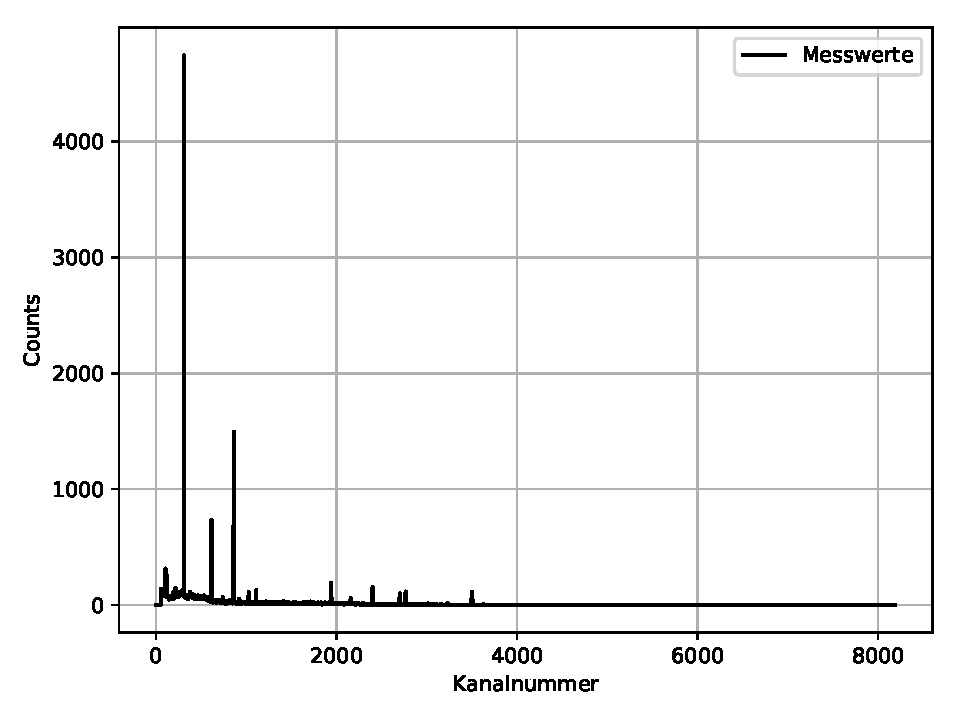
\includegraphics[height=7cm]{plot1.pdf}
  \caption{Halblogarithmisch aufgetragene Messwerte für Ag mit Ausgleichsgeraden.}
  \label{fig:plot1}
\end{figure}

Aus Gleichung \ref{eqn:lnN} kann entnommen werden, dass die Steigungen der Ausgleichsgeraden
gerade der Zerfallskonstante $\lambda$ entsprechen, da $ln(N_0(1-\exp{(-\lambda\Delta t)}))$
eine Konstante ist kann auch
\begin{equation}
  ln(N_{\Delta t}(t))= -\lambda t +b
  \label{eqn:gerade}
\end{equation}
geschrieben werden.
Es werden folgende Geradensteigungen ermittelt:
\begin{align*}
  \lambda_{\text{ges}}=\SI{11,22(82)e-3}{\per\s}\\
  \lambda_{\text{lang}}=\SI{1,50(137)e-3}{\per\s}\\
  \lambda_{\text{kurz}}=\SI{9,7(16)e-3}{\per\s}\\
\end{align*}
Somit lauten die dazugehörigen Geradengleichungen:

\begin{align*}
  ln(N_{\Delta t\;\text{ges}}(t))&=\SI{11,22(82)e-3}{\per\s}\cdot t+(\SI{4,73(11)}{})\\
  ln(N_{\Delta t\;\text{lang}}(t))&=\SI{1,50(137)e-3}{\per\s}\cdot t +(\SI{2,68(47)}{})\\
  ln(N_{\Delta t\;\text{kurz}}(t))&=\SI{9,7(16)e-3}{\per\s}\cdot + (\SI{2,0(5)}{})
\end{align*}

Nach Formel \ref{eqn:gerade} entspricht $ln(N_0(1-\exp{[-\lambda\Delta t]}))$ gerade $b$, somit folgt:
\begin{align*}
  N_{0,kurz}(1-\exp{[-\lambda\Delta t]})=\SI{10(7)}{}\\
  N_{0,lang}(1-\exp{[-\lambda\Delta t]})=\SI{12(8)}{}\\
  N_{0,ges}(1-\exp{[-\lambda\Delta t]})=\SI{114(13)}{}\\
\end{align*}

Aus den Zerfallskonstanten lassen sich nach Gleichung \ref{eqn:zkonst} die Halbwertszeiten berechnen:
\begin{align*}
  T_{ges}=\SI{62(5)}{\s}\\
  T_{lang}=\SI{500(400)}{\s}\\
  T_{kurz}=\SI{71(12)}{\s}\\
\end{align*}

Um zu zeigen, dass die Relation
\begin{equation}
  N_{\Delta t,\text{kurz}}(t_i) <<N_{\Delta t,\text{lang}}(t_i)
\end{equation}
gilt, werden die Werte an der Stelle $t^{*}$ berechnet.
\begin{align}
  N_{\Delta t,\text{kurz}}(t^{*}) &<<N_{\Delta t,\text{lang}}(t^{*})\\
  \SI{0,1(6)}{}&<<\SI{2,4(5)}{}\\
\end{align}
Da die Steigungen beide negativ sind, ist diese Ungleichung also immer erfüllt, wenn sie
am Ort $t^{*}$ erfüllt ist.

Zuletzt werden die Summenkurve aus den errechneten Werten zusammen mit den Messwerten in
einem Diagramm dargestellt, dies ist in Abbildung \ref{fig:plot4} zu sehen.
\begin{figure}[H]
  \centering
  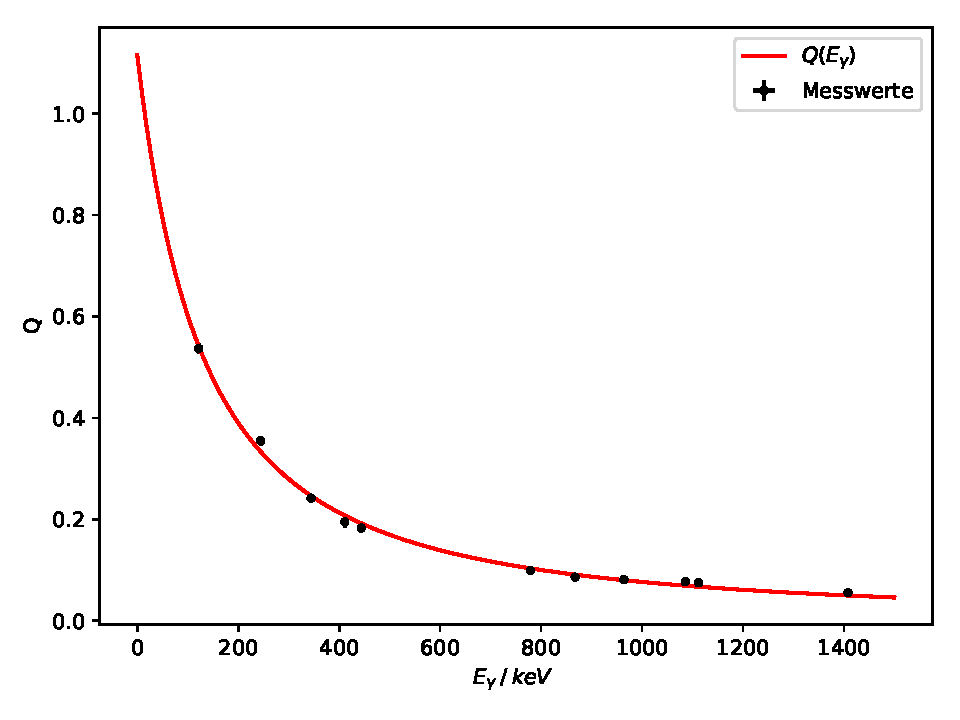
\includegraphics[height=7cm]{plot4.pdf}
  \caption{Summenkurve zusammen mit den Messwerten.}
  \label{fig:plot4}
\end{figure}

%Indium
Für Indium, dessen Messwerte in Tabelle \ref{tab:tab2} zu sehen sind, wird ähnlich vorgegangen.
Die Messwerte werden werden mit Fehlerbalken und Ausgleichsgerade halblogarithmisch
aufgetragen, dies ist in Abbildung \ref{fig:plot2} dargestellt ist.
\begin{table}[H]
  \centering
  \caption{Wertetabelle für $\alpha$ und $C_V$.}
  \label{tab:tab2}
    \begin{tabular}{S S S S S}
    \toprule
    $ T\: \text{in}\: \si{\K} $ & $ {\alpha \cdot 10^{-6} \: \text{in}\: \si {\per\K}} $ &
    $ C_V \: \text{in}\: \si{\J\per\K\mol} $\\
    \midrule %Cv, a *10-6, Cv
    %0 & 1 & 1\\
    88.60\pm0.24 & 9.56\pm0.06 & 14.17\pm8.13  \\ %&3.6 & 318.97\pm0.85\\
    93.81\pm0.24 & 10.10\pm0.06 & 17.58\pm10.03 \\ %& 4.7 & 440.90\pm1.11\\
    99.74\pm0.24 & 10.66\pm0.05 & 15.52\pm8.84 \\ %& 5.1 & 508.68\pm1.21\\
    104.74\pm0.24 & 11.07\pm0.05 & 18.44\pm10.52 \\ %& 4.6 & 481.79\pm1.09\\
    110.94\pm0.24 &  11.54\pm0.05 & 14.86\pm8.45 \\ %& 5.3 & 587.97\pm1.27\\
    115.96\pm0.24 & 11.89\pm0.05 & 18.49\pm10.52 \\ %& 4.6 & 533.41\pm1.10\\
    121.47\pm0.24 &  12.22\pm0.05 & 16.83\pm9.57 \\ %& 4.9 & 595.21\pm1.17\\
    126.99\pm0.24 & 12.53\pm0.04 & 16.79\pm9.54 \\ %& 4.9 & 622.29\pm1.18\\
    131.58\pm0.24 & 12.77\pm0.04 & 20.42\pm11.62 \\ %& 4.2 & 552.62\pm1.01\\
    136.65\pm0.24 & 13.02\pm0.04 & 18.40\pm10.47 \\ %& 4.6 & 628.57\pm1.11\\
    141.49\pm0.24 & 13.24\pm0.04 & 19.28\pm10.97 \\ %& 4.4 & 622.54\pm1.07\\
    146.34\pm0.24 & 13.44\pm0.04 & 19.24\pm10.95 \\ %& 4.4 & 643.88\pm1.07\\
    150.95\pm0.24 & 13.62\pm0.04 & 20.22\pm11.52 \\ %& 4.3 & 649.11\pm1.05\\
    155.34\pm0.24 & 13.79\pm0.04 & 21.31\pm12.14 \\ %& 4.1 & 636.88\pm0.98\\
    159.97\pm0.24 & 13.95\pm0.04 & 20.12\pm11.47 \\ %& 4.3 & 687.89\pm1.05\\
    164.62\pm0.24 & 14.10\pm0.04 & 20.18\pm11.51 \\ %& 4.3 & 707.87\pm1.06\\
    168.79\pm0.25 & 14.23\pm0.04 & 22.54\pm12.86 \\ %& 3.9 & 658.27\pm0.95\\
    173.45\pm0.25 &  14.37\pm0.04 & 20.08\pm11.46 \\ %& 4.3 & 745.84\pm1.06\\
    178.13\pm0.25 &  14.50\pm0.04 & 20.04\pm11.44 \\ %& 4.3 & 765.94\pm1.06\\
    182.56\pm0.25 &  14.62\pm0.04 & 21.11\pm12.06\\
    192.70\pm0.25 &  14.87\pm0.04 & 18.41\pm10.47\\
    200.15\pm0.25 &  15.04\pm0.04 & 25.19\pm14.28\\
    208.87\pm0.25 &  15.23\pm0.04 & 21.43\pm12.18\\
    217.12\pm0.25 &  15.38\pm0.04 & 22.65\pm12.88\\
    225.15\pm0.25 &  15.53\pm0.03 & 23.27\pm13.24\\
    232.70\pm0.25 &  15.70\pm0.03 & 24.75\pm14.08\\
    240.53\pm0.25 &  15.74\pm0.03 & 23.84\pm13.58\\
    248.39\pm0.25 &  15.89\pm0.03 & 23.74\pm13.53& \\
    256.01\pm0.25 &  15.97\pm0.03 & 24.46\pm13.94 \\
    263.41\pm0.26 &  16.01\pm0.03 & 25.22\pm14.38 \\
    271.08\pm0.26 &  16.18\pm0.03 & 24.26\pm13.86 \\
    278.52\pm0.26 &  16.27\pm0.03 & 25.03\pm14.29&\\
    285.98\pm0.26 &  16.35\pm0.03 & 24.92\pm14.25 \\
    293.21\pm0.26 &  16.42\pm0.03 & 25.74\pm14.72 \\
    300.98\pm0.26 &  16.50\pm0.03 & 23.87\pm13.68 \\
    308.51\pm0.26 &  16.57\pm0.03 & 24.63\pm14.12\\



      \bottomrule
    \end{tabular}
\end{table}


\begin{figure}[H]
  \centering
  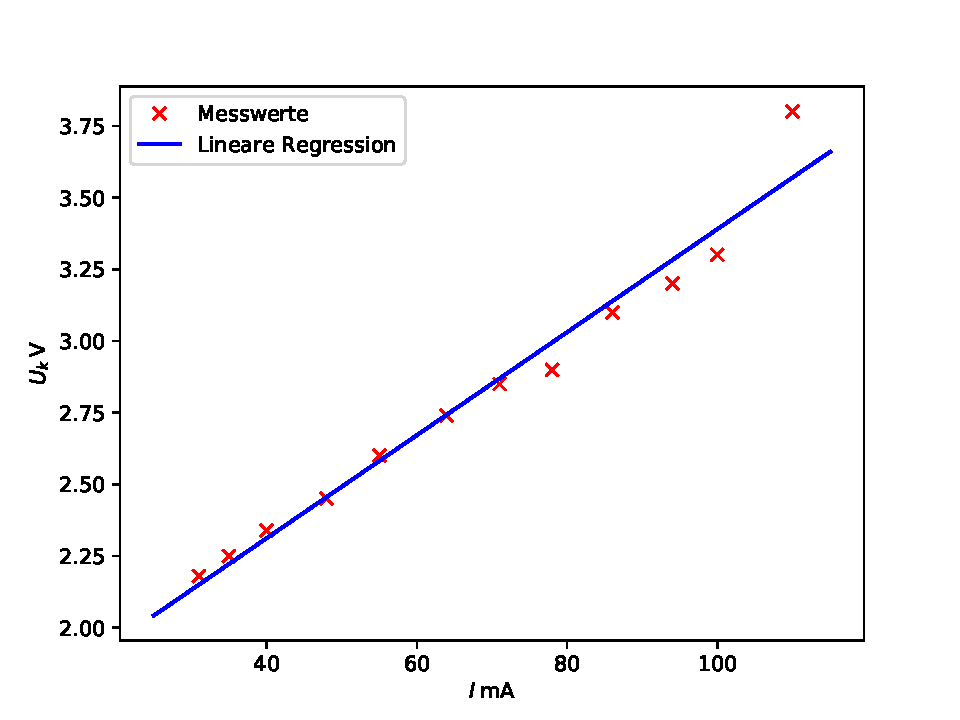
\includegraphics[height=7cm]{plot2.pdf}
  \caption{Messwerte für Indium mit Fehlerbalken und Ausgleichsgerade.}
  \label{fig:plot2}
\end{figure}

Die so ermittelte Geradengleichung lautet:

\begin{equation*}
  N_{\Delta t}(t)=\SI{23,1(94)e-5}{\per\s}\cdot t + (\SI{7,81(2)}{})
\end{equation*}

Der Vergleich mit Gleichung \ref{eqn:gerade} zeigt, dass die Größe
$ln(N_0(1-\exp{[-\lambda\Delta t]}))$ gerade dem y-Achsenabschnitt entspricht.
Daraus folgt, dass
\begin{equation*}
  N_0(1-\exp{[-\lambda\Delta t]})=\SI{2,47(5)e+3}{}
\end{equation*}

Äquivalent zur vorherigen Rechnung ergibt sich aus der Zerfallskonstante $\lambda$, bzw. der
Steigung der Geraden nach Formel \ref{eqn:zkonst} die Halbwertszeit
\begin{equation*}
  T=\SI{3,01(012)e+3}{\s}.
\end{equation*}
